\documentclass{beamer}
\usefonttheme{professionalfonts}% font de LaTeX
\usetheme{Warsaw} % Tema de la presentación
\mode<presentation>
%%%% packages  %%%%
\usepackage[utf8]{inputenc}
\usepackage[spanish]{babel}
\usepackage{amsmath, amsthm, amsfonts}
\usepackage{verbatim}
\usepackage{graphicx}
\usepackage{subfigure}
\usepackage{xcolor}
\usepackage{colortbl}
\usepackage{listings} 
% \lstset{escapeinside={<*}{*>}}
\lstdefinestyle{base}{
  language=java,
  emptylines=1,
  breaklines=true,
  basicstyle=\footnotesize,
  moredelim=**[is][\color{red}]{@}{@},
  moredelim=**[is][\color{blue}]{-}{-},
  moredelim=**[is][\color{green}]{<}{>},
  }
\graphicspath{{../imagenes/}}
%\usepackage[table]{xcolor}
\begin{document}
\title[FLUJO DE INFORMACIÓN EN APLICACIONES ANDROID]{ANÁLISIS DE FLUJO DE
    INFORMACIÓN EN APLICACIONES ANDROID}
    \author{\textbf{Lina Marcela Jiménez Becerra}}
    \institute[Universities Here and There]{
    	UNIVERSIDAD DE LOS ANDES \newline
    	DEPARTAMENTO DE INGENIERÍA DE SISTEMAS Y COMPUTACIÓN }
    \date{Junio 9, 2015}
    \frame{\titlepage}
	\section{Background}
\subsection{}
\begin{frame}{Background}
	\begin{block}{Técnicas de análisis}
	\begin{itemize}
	  \item Análisis estático. \pause 
	  \item Análisis dinámico. \pause
	  \item Security Typed languages.
	\end{itemize}
	\end{block}
\end{frame}
\begin{frame}{Background}
	\begin{block}{Aplicaciones Android}
	\begin{itemize}
	  \item Aplicación Java con interfaces descritas en XML.
	  \item Framework Android.
	  \item Componentes de aplicación.
	\end{itemize}
	\pause
	\end{block}
	\begin{block}{Sistema de anotaciones en Jif}
	\begin{itemize}
	  \item Lenguaje tipado de seguridad.
	  \item Extensiones de seguridad para el lenguaje Java.
	  \item Restricciones para uso de la información.
	  \item Label checking.
	\end{itemize}
	\end{block}
\end{frame}
\begin{frame}{Background}
	\begin{block}{DML de JIF}
		Elementos del modelo de anotación:
		\begin{itemize}
		  \item Principals
		  \item Políticas
		  \item Labels
		\end{itemize}
	\end{block}
\end{frame}
\begin{frame}[fragile]{Background}
% 	\pause
	\begin{block}{Principals}
		Autoridad sobre un sistema o programa(Alice, Bob, Chunck)
	\end{block}
	\pause
	\begin{block}{Políticas}
		\{owner: reader list\}\ u \{owner: writer list\}
	\end{block}
	\pause
	\begin{block}{Labels} 
		Políticas de seguridad que se adicionan a las expresiones del programa.
		\begin{lstlisting}[style=base]
			int@{Alice:}@ code;
		\end{lstlisting}
	\end{block}
\end{frame}
	 \section{Descripción del Problema}

\begin{frame}{Descripción del Problema}
	\begin{block}{Manipulación de información del usuario}
	\begin{itemize}
	\item El desarrollador Android no tiene cómo definir políticas de seguridad para
	regular el flujo de información de sus aplicaciones.
	\item Complejidad para prevenir fugas de información del usuario.
	\end{itemize}
	\end{block}
	\pause
	\begin{block}{Reporte McAffe}
	\begin{itemize}
	\item Aplicaciones Android invasivas de la privacidad del usuario.
	\item No toda aplicación invasiva contiene malware.
	\item De las aplicaciones que más vulneran la privacidad del usuario 35 \%
	contienen malware.
	\end{itemize}
	\end{block}
\end{frame}

\begin{frame}{Descripción del Problema}
\begin{block}{Limitaciones de la API}
\begin{itemize}
  \item Políticas de control de acceso de la API.
  \item Regular el acceso a recursos protegidos.
  \item No hacen seguimiento al flujo de información.
\end{itemize}
\end{block}
\begin{block}{Propuestas existentes}
\begin{itemize}
  \item Análisis estático y análisis dinámico.
  \item Análisis dinámico: actuales caminos de ejecución.
  \item Análisis estático: es posible incluir todos los caminos de ejecución.
\end{itemize}
\end{block}
\end{frame}

\begin{frame}{Descripción del Problema}
\begin{block}{Propuestas existentes}
Data-Flow con técnicas de análisis tainting.
\begin{itemize}
	  \item Se hace seguimiento a los datos marcados.
	  \item No incluye todos los posibles caminos de ejecución.
	  \item Ejemplo: FlowDroid
\end{itemize}
\end{block}
\end{frame}
% 
\begin{frame}{Descripción del Problema}
\begin{block}{Propuestas existentes}
Flujo de información con técnicas Program Dependence Graphs(PDG).
\begin{itemize}
 	  \item Los PDG proveen una representación del programa que se analiza.
	  \item Análisis de flujos de información del programa de principio a fin.
	  \item Incluye todos los posibles caminos de ejecución.
	  \item Ejemplo: Joana.
\end{itemize}
\end{block}
\end{frame}

\begin{frame}{Descripción del Problema}
\begin{block}{Propuestas existentes}
Enfoque de las propuestas existentes:
\begin{itemize}
  \item Identificar fugas de información en aplicativos ya implementados.
  \item FlowDroid: no incluye todos los posibles caminos de ejecución.
  \item Joana: no permite definir las políticas de seguridad a evaluar.
\end{itemize}
\end{block}
\end{frame}
% 
% 
% \begin{frame}{Descripción del Problema}
% \begin{block}{Propuestas existentes limitaciones}
% 	
% \end{block}
% \begin{block}{Propuestas existentes limitaciones}
% 
% \end{block}
% \end{frame}
 
	 \section{Propuesta}
\subsection{Requerimientos}
\begin{frame}{Propuesta de solución}
	\begin{block}{El desarrollador requiere}
		\begin{itemize}
		  \item Definir políticas de seguridad desde la implementación de sus aplicativos.
		  \item Una herramienta que verifique las políticas definidas.
		  \item Garantizarle al usuario que la aplicación respeta determinadas
		  políticas de seguridad.
		\end{itemize}
	\end{block}
\end{frame}

\subsection{Propuesta - Generalidades}
\begin{frame}{Propuesta de solución}
	\begin{block}{Propuesta}
		  Proveer una herramienta de análisis de flujo de información mediante el
		  sistema de anotaciones de Jif.
	\end{block}
	\center{Herramienta de Análisis Estático}
	\begin{figure}[t!]
		\begin{center} 
		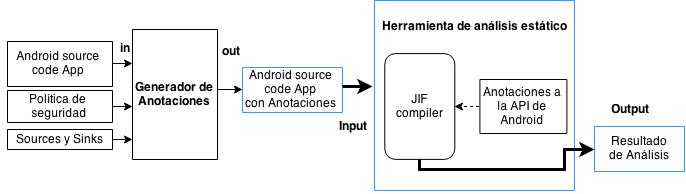
\includegraphics[width=9cm]{desing3Real-2-2-azul.jpg} 
		\end{center}
	\end{figure}
\end{frame}

\subsection{Jif}
\begin{frame}{Características de Jif}
\begin{itemize}
  \item Lenguaje tipado de seguridad.
  \item Extensiones de seguridad al lenguaje java.
  \item Restricciones para uso de la información.
  \item Análisis de flujo de información mediante chequeo de etiquetas.
\end{itemize}
\end{frame}
\begin{frame}[fragile]{Características sobresalientes de Jif}
\begin{columns}[T]
\column{2in}
	\begin{itemize}
	  \item Anotar propiedades de seguridad.
	  \item Verificar las propiedades de seguridad.
	  \item Cubrir todas las posibles ramas de ejecución en el análisis.
	  \item Diseñado para aplicativos Java.
	\end{itemize}
\column{2in}{Flujos: explicitos - implícitos }
\begin{lstlisting}[style=base]
	int x,y;
	x = 1;	
	y = 4 + x;
\end{lstlisting}
\begin{lstlisting}[style=base]
	void foo(a){
	int x;
	if(a > 10)
		x = 1;
	else
		x = 2;
	printf(x);
	}
\end{lstlisting}
\end{columns}

\end{frame}

\subsection{Propuesta - Especificaciones}
\begin{frame}[fragile]{Política de Seguridad}
\begin{columns}[T]
\column{1.5in}
	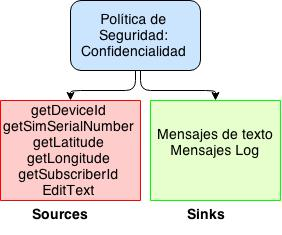
\includegraphics[width=4cm]{Politica.jpg} 
	\pause
\column{2.5in}
\begin{lstlisting}[style=base]
	String imei = @getDeviceId()@;
	<sendTextMessage>(imei);
\end{lstlisting}
\pause
\begin{lstlisting}[style=base][frame=single]
String passwd = @EditText@.getText();
boolean passwdOk = false;
if(passwd.equals("superSecure"))
	passwdOk = true;
if(passwdOk)
	<Log>.i("INFO","Password correcto");
else
	<Log>.i("INFO","Password incorrecto");
\end{lstlisting}
% \begin{lstlisting}[style=base][frame=single]
% String passwd = @EditText@.getText();
% boolean passwdOk = false;
% if(passwd.equals("superSecure"))
% 	passwdOk = true;
% 	
% if(passwdOk)
% 	<Log>.i("INFO","Password correcto");
% else
% 	<Log>.i("INFO","Password incorrecto");
% \end{lstlisting}
\end{columns}
\end{frame}

\begin{frame}[fragile]{Anotaciones Propuestas}
\begin{columns}[T]
\column{1.5in}{DLM de Jif}
\begin{mdframed}
\scriptsize{
\textbf{Principales}\newline
Autoridad
}
\end{mdframed}
\vspace{-0.5em}
\begin{mdframed}
\scriptsize{
\textbf{Políticas}\newline
{dueño: lista-lectores}
}
\end{mdframed}
\vspace{-0.5em}
\begin{mdframed}

\scriptsize{
\textbf{Etiquetas}\newline}
\begin{lstlisting}[style=base2][
int code; 
int {Alice:} code; 
\end{lstlisting}
\end{mdframed}
\vspace{-0.5em}
\column{2in}
\begin{mdframed}
\scriptsize{
\textbf{Autoridad máxima}\newline
El Principal \emph{\textcolor{red}{Alice}} representa la máxima autoridad del
programa.}
\end{mdframed}
\vspace{-0.5em}

\begin{mdframed}
\scriptsize{
\textbf{Política para anotar información con nivel de seguridad alto:}
\vspace{-0.5em}
\begin{lstlisting}[style=base2]
@{Alice:}@
\end{lstlisting}
\vspace{-0.5em}
Sólo la autoridad máxima del programa podrá leer la información. 
}
\end{mdframed}
\vspace{-0.5em}

\begin{mdframed}
\scriptsize{
\textbf{Política para anotar información con nivel de seguridad bajo:}
\vspace{-0.5em}
\begin{lstlisting}[style=base2]
<{ }>
\end{lstlisting}
\vspace{-0.5em}
No se define un Principal la información podrá leerse por todos. }
\end{mdframed}
\end{columns}
\end{frame}

\begin{frame}{Anotaciones a la API} 
\begin{block}{Flujo de información en la API}
	\begin{itemize}
	  \item La API posibilita el acceso de la app a sources y Sinks.
	  \item Se generan flujos de información.
	  \item Controlar flujos de información entre sources y sinks.
	\end{itemize}
\end{block}
\begin{block}{Sources y sinks definidos en la API}
	\begin{itemize}
	  \item getDeviceId (método source) $\rightarrow$ TelephonyManager
	  \item Mensajes de texto (sinks) $\rightarrow$ SmsManager
	\end{itemize}
\end{block}
\end{frame}

\begin{frame}[fragile]{Anotaciones a la API}
\begin{block}{Flujo explícito}
\begin{center}
\begin{lstlisting}[style=base2]
String @{Alice:}@imei = getDeviceId();
String <{}> pub = imei;
\end{lstlisting}
\end{center}
\end{block}

\begin{block}{Flujo implícito}
\begin{center}
\begin{lstlisting}[style=base2][frame=single]
String @{Alice:}@passwd = EditText.getText();
boolean <{}>passwdOk = false;
if(passwd.equals("superSecure"))
	passwdOk = true;
	
if(passwdOk)
	<Log>.i("INFO","Password correcto");
else
	<Log>.i("INFO","Password incorrecto");
\end{lstlisting}
\end{center}
\end{block}
\end{frame}

	 \section{Resultados de evaluación}
	
\begin{frame}{Evaluación}
	\begin{block}{}
	Comparación con FlowDroid y JoDroid
	\end{block}
\end{frame}
	 \section{Conclusiones}
	
\begin{frame}{Conclusiones}
\begin{block}{}
	\begin{itemize}
		\item Se dan los primeros pasos para el análisis de flujo de
		información de aplicaciones Android mediante Jif.\pause
		\item El desarrollador obtiene las ventajas de bajo costo en desempeño.\pause
		\item Análisis de flujos implícitos.\pause
		\item Desempeño y completitud en el análisis.\pause
		\item Retos para el análisis de aplicaciones Android mediante el sistema de
		anotaciones de Jif.
	\end{itemize}
\end{block}
\end{frame}
	 \section{Trabajo Futuro}
	
\begin{frame}{Trabajo Futuro}
	\begin{block}{}
	\begin{itemize}
	  \item Extensiones al esquema de anotación.
	  \item Análisis de políticas de integridad.
	  \item Mecanismos adicionales: declasificación y endorsement.
	\end{itemize}
	\end{block}
\end{frame}

\begin{frame}{Preguntas}

\end{frame}
\end{document}
